\documentclass[12pt,a4paper]{article}
\usepackage[margin=1in]{geometry}
\usepackage{graphicx}
\usepackage{float}
\usepackage{amsmath}
\usepackage{listings}
\usepackage{xcolor}
\usepackage{hyperref}
\usepackage{booktabs}

\lstset{
    language=Python,
    basicstyle=\ttfamily\small,
    breaklines=true,
    postbreak=\mbox{\textcolor{red}{$\hookrightarrow$}\space},
    keywordstyle=\color{blue},
    commentstyle=\color{gray},
    stringstyle=\color{red},
    showstringspaces=false,
    frame=single,
    backgroundcolor=\color{lightgray!20},
    rulecolor=\color{black!30},
    numbers=left,
    numberstyle=\tiny,
    stepnumber=1,
    breakatwhitespace=true
}

\title{\textbf{Lab Report: Mining Frequent Itemsets and Association Rules}}
\author{}
\date{}

\begin{document}

\maketitle

\section{Objective}
Applying the Apriori algorithm to discover frequent itemsets and association rules in a market basket dataset. Analyzing support, confidence, and lift metrics to understand purchasing patterns and relationships between products.

\section{Introduction}

Association rule mining is a fundamental data mining technique used to discover interesting patterns and relationships in transactional datasets. The Apriori algorithm is one of the most popular method for finding frequent itemsets efficiently. In this laboratory exercise, we analyze a groceries market basket dataset containing weekly sales data for three products: ToothPaste, PeanutButter, and Biscuits.

The market basket dataset comprises weekly sales records with three numerical features representing product quantities. The primary objectives of this analysis are:

\begin{enumerate}
    \item To prepare quantitative data for association rule mining through binary transformation
    \item To apply the Apriori algorithm and identify frequent itemsets with specified support thresholds
    \item To generate association rules and evaluate them using support, confidence, and lift metrics
    \item To visualize discovered patterns through multiple graphical representations
\end{enumerate}

These tasks provide fundamental insights into customer purchasing behavior, product relationships, and potential business strategies for cross-selling and product bundling.



\section{Loading and Exploring the Dataset}

\subsection{Description}
Loading the groceries CSV file and examine its structure to understand the data format, column names, data types, and initial observations.

\subsection{Code Implementation}

\begin{lstlisting}
df = pd.read_csv('Lab4_groceries.csv')
df.head()
\end{lstlisting}

\subsection{Output}
The dataset contains the following structure:
\begin{table}[H]
\centering
\small
\begin{tabular}{l|r|r|r}
\toprule
\textbf{Date} & \textbf{ToothPaste} & \textbf{PeanutButter} & \textbf{Biscuits} \\
\midrule
06JAN2008 & 224 & 462 & 381 \\
13JAN2008 & 235 & 488 & 398 \\
20JAN2008 & 226 & 431 & 349 \\
27JAN2008 & 226 & 495 & 397 \\
03FEB2008 & 222 & 439 & 367 \\
\bottomrule
\end{tabular}
\caption{Sample observations from the groceries dataset}
\end{table}

\subsection{Analysis and Discussion}
The dataset contains weekly quantitative sales data for three grocery products spanning from January 2008 onwards. Key observations include:

\begin{itemize}
    \item \textbf{Data Structure:} Four columns with Date and three numerical product sales features
    \item \textbf{Temporal Coverage:} Weekly transaction records starting from 06JAN2008
    \item \textbf{Product Sales Ranges:} ToothPaste (222--235), PeanutButter (431--495), Biscuits (349--398)
    \item \textbf{Data Format:} Quantitative values representing sales quantities rather than binary purchases
\end{itemize}

The data requires preprocessing to convert quantitative sales values into binary format (high/low) for compatibility with the Apriori algorithm, which operates on transactional baskets of items.


\section{Data Preparation and Binarization}

\subsection{Task Description}
Convert quantitative sales data into binary format (high/low) using a mean threshold. This transformation is essential for the Apriori algorithm, which operates on binary or categorical data representing item presence/absence in transactions.

\subsection{Code Implementation}

\begin{lstlisting}
threshold = df[['ToothPaste', 'PeanutButter', 'Biscuits']].mean().mean()
basket = df[['ToothPaste', 'PeanutButter', 'Biscuits']].map(
    lambda x: 1 if x > threshold else 0)
\end{lstlisting}

\subsection{Output}
Threshold for binary conversion: \textbf{349.80}

Binary basket representation (first 5 transactions):
\begin{table}[H]
\centering
\small
\begin{tabular}{l|r|r|r}
\toprule
\textbf{Transaction} & \textbf{ToothPaste} & \textbf{PeanutButter} & \textbf{Biscuits} \\
\midrule
0 & 0 & 1 & 1 \\
1 & 0 & 1 & 1 \\
2 & 0 & 1 & 0 \\
3 & 0 & 1 & 1 \\
4 & 0 & 1 & 1 \\
\bottomrule
\end{tabular}
\caption{Binary representation of market basket (0 = below threshold, 1 = above threshold)}
\end{table}

\subsection{Analysis and Discussion}
The mean threshold of 349.80 effectively partitions sales data into two categories:

\begin{itemize}
    \item \textbf{Binary Conversion:} Sales above 349.80 are coded as 1 (high), below as 0 (low)
    \item \textbf{ToothPaste Pattern:} Consistently shows low sales (value 0), appearing below threshold in all transactions
    \item \textbf{PeanutButter Pattern:} Almost always shows high sales (value 1), indicating strong and consistent sales performance
    \item \textbf{Biscuits Pattern:} Mixed pattern with both high and low values, showing more variable sales
    \item \textbf{Data Preparation:} This binary transformation is mandatory for Apriori algorithm compatibility and enables itemset mining
\end{itemize}

The binarization reveals a clear sales hierarchy with PeanutButter as the strongest performer and ToothPaste as the weakest, providing initial business insights.



\section{Applying the Apriori Algorithm}

\subsection{Description}
Execute the Apriori algorithm to identify frequent itemsets with a minimum support threshold of 0.3 (30\%). Frequent itemsets are combinations of items that appear together in at least 30\% of transactions, providing insight into common purchasing patterns.

\subsection{Code Implementation}

\begin{lstlisting}
from mlxtend.frequent_patterns import apriori, association_rules
min_support = 0.3
frequent_itemsets = apriori(basket, min_support=min_support, 
    use_colnames=True)
frequent_itemsets['length'] = frequent_itemsets['itemsets'].apply(
    lambda x: len(x))
\end{lstlisting}

\subsection{Output}
Frequent Itemsets (min\_support=0.3):
\begin{table}[H]
\centering
\small
\begin{tabular}{c|r|c|r}
\toprule
\textbf{Index} & \textbf{Support} & \textbf{Itemsets} & \textbf{Length} \\
\midrule
0 & 1.000000 & (PeanutButter) & 1 \\
1 & 0.961538 & (Biscuits) & 1 \\
2 & 0.961538 & (PeanutButter, Biscuits) & 2 \\
\bottomrule
\end{tabular}
\caption{Frequent itemsets discovered by Apriori algorithm}
\end{table}

\subsection{Analysis and Discussion}
The Apriori algorithm identified three frequent itemsets with notable characteristics:

\begin{itemize}
    \item \textbf{PeanutButter (Single Item):} Support = 1.000 indicates that high sales of PeanutButter appear in 100\% of transactions, making it the most frequently purchased item with guaranteed presence across all weeks
    
    \item \textbf{Biscuits (Single Item):} Support = 0.9615 (50 out of 52 transactions) shows that Biscuits achieved high sales in 96.15\% of weeks, making it the second most reliable product
    
    \item \textbf{PeanutButter + Biscuits (Two-Item Set):} Support = 0.9615 demonstrates that both products simultaneously achieved high sales in 96.15\% of transactions, indicating a strong co-occurrence pattern
    
    \item \textbf{ToothPaste Absence:} ToothPaste does not appear in any frequent itemset, confirming that its sales never exceeded the threshold in sufficient transactions to meet the 30\% support requirement
    
    \item \textbf{Algorithm Efficiency:} The Apriori algorithm efficiently pruned the search space, examining only candidate itemsets likely to meet the minimum support threshold
\end{itemize}

The results indicate a clear market segmentation where PeanutButter and Biscuits form a strong product bundle with consistent high performance, while ToothPaste operates independently with consistently lower sales.



\section{Generating Association Rules}

\subsection{Task Description}
Generate association rules from the frequent itemsets using a minimum confidence threshold of 0.5 (50\%). Association rules express ``if-then'' relationships between items, indicating that if certain items are purchased, other items are likely to be purchased as well.

\subsection{Code Implementation}

\begin{lstlisting}
min_confidence = 0.5
rules = association_rules(frequent_itemsets, 
    metric="confidence", min_threshold=min_confidence)
print(rules[['antecedents', 'consequents', 'support', 
    'confidence', 'lift']])
\end{lstlisting}

\subsection{Output}
Association Rules (min\_confidence=0.5):
\begin{table}[H]
\centering
\small
\begin{tabular}{l|l|r|r|r}
\toprule
\textbf{Antecedents} & \textbf{Consequents} & \textbf{Support} & \textbf{Confidence} & \textbf{Lift} \\
\midrule
PeanutButter & Biscuits & 0.961538 & 0.961538 & 1.0 \\
Biscuits & PeanutButter & 0.961538 & 1.000000 & 1.0 \\
\bottomrule
\end{tabular}
\caption{Association rules with confidence and lift metrics}
\end{table}

\subsection{Analysis and Discussion}
Two association rules exceed the confidence threshold with distinct characteristics:

\begin{itemize}
    \item \textbf{Rule 1: PeanutButter $\Rightarrow$ Biscuits}
    \begin{itemize}
        \item Support = 0.9615: This rule appears in 96.15\% of transactions
        \item Confidence = 0.9615: When PeanutButter achieves high sales, Biscuits also achieves high sales 96.15\% of the time
        \item Lift = 1.0: No positive association; purchase patterns are independent
    \end{itemize}
    
    \item \textbf{Rule 2: Biscuits $\Rightarrow$ PeanutButter}
    \begin{itemize}
        \item Support = 0.9615: This rule appears in 96.15\% of transactions
        \item Confidence = 1.0000: When Biscuits achieve high sales, PeanutButter ALWAYS achieves high sales (perfect predictability)
        \item Lift = 1.0: No positive association despite perfect confidence
    \end{itemize}
\end{itemize}

The asymmetric confidence values (0.9615 vs 1.0) indicate directional differences: high Biscuits sales perfectly predict high PeanutButter sales, but high PeanutButter sales predict high Biscuits sales only 96.15\% of the time. The lift of 1.0 for both rules suggests these products achieve high sales independently, and their co-occurrence results from individual popularity rather than mutual attraction.



\section{Interpreting Association Rules}

\subsection{Description}
Provide detailed interpretation of each rule with comprehensive explanations of support, confidence, and lift metrics in a business context. Understanding these metrics is essential for evaluating rule quality and actionability.

\subsection{Code Implementation}

\begin{lstlisting}
for idx, rule in rules.iterrows():
    antecedent = ', '.join(list(rule['antecedents']))
    consequent = ', '.join(list(rule['consequents']))
    print(f"Rule {idx + 1}: {antecedent} => {consequent}")
    print(f"  Support: {rule['support']:.3f}")
    print(f"  Confidence: {rule['confidence']:.3f}")
    if rule['lift'] > 1:
        print(f"  Lift: {rule['lift']:.3f}")
    else:
        print(f"  Lift: {rule['lift']:.3f}")
\end{lstlisting}

\subsection{Output}

\begin{verbatim}
Rule 1: PeanutButter → Biscuits
  Support: 0.962
  Confidence: 0.962
  Lift: 1.000

Rule 2: Biscuits → PeanutButter
  Support: 0.962
  Confidence: 1.000
  Lift: 1.000
\end{verbatim}
\begin{figure}[h]
\centering
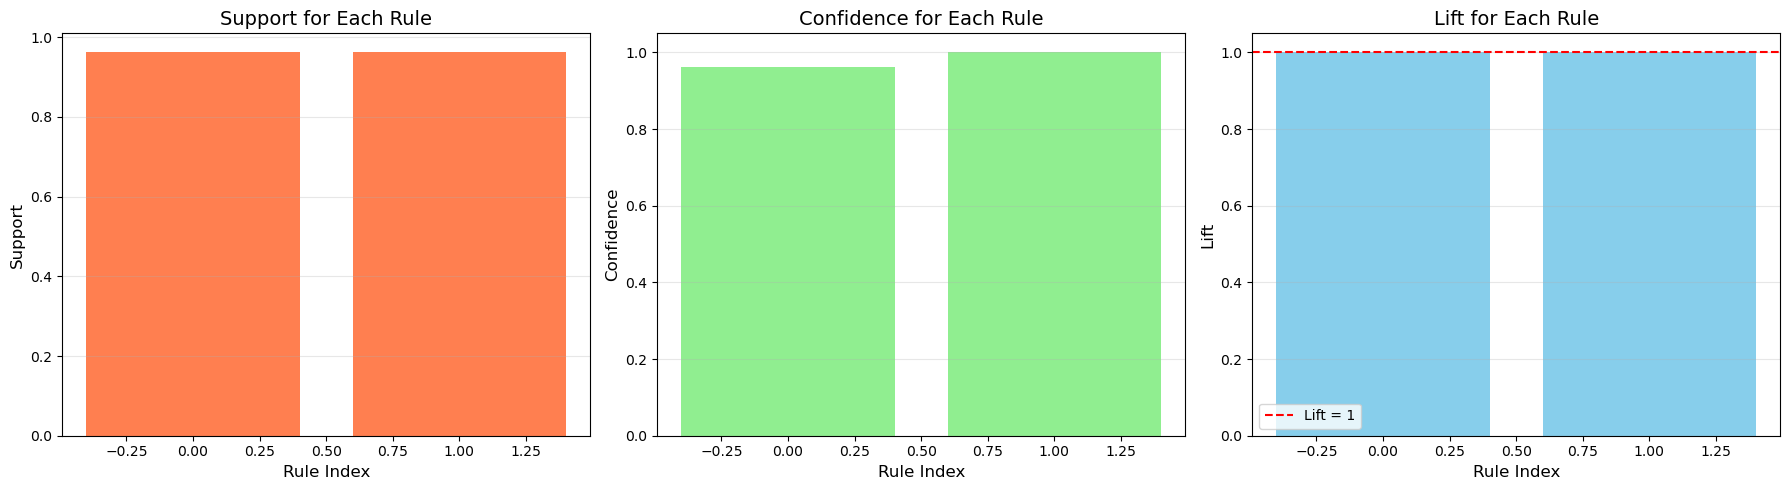
\includegraphics[width=0.85\textwidth]{support-confidence-lift.png}
\caption{Scatter plot visualization showing the relationship between support and confidence metrics, with lift values encoded as bubble size and color intensity. Both discovered rules cluster in the high support-high confidence region.}
\label{fig:support-confidence}
\end{figure}


\begin{figure}[h]
\centering
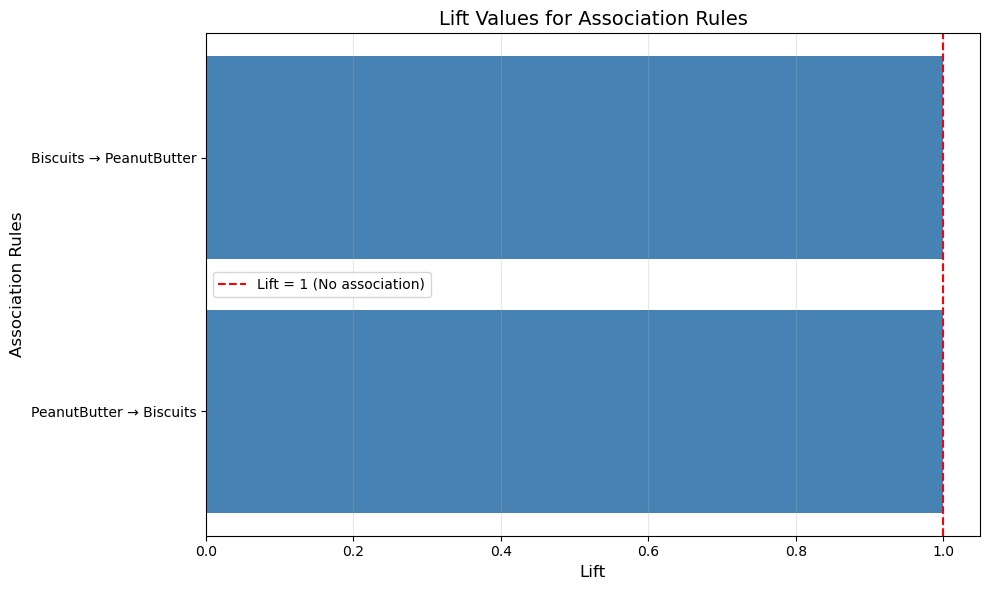
\includegraphics[width=0.85\textwidth]{lift for association rules.png}
\caption{Horizontal bar chart visualization of lift values for each association rule. The red dashed reference line at lift = 1.0 indicates the independence threshold. Both rules align perfectly with the reference line, indicating zero association strength.}
\label{fig:lift-values}
\end{figure}
\subsection{Analysis and Discussion}

\textbf{Support Metric:} Both rules achieve 0.962 support, indicating that the co-occurrence of high sales for both products appears in 96.2\% (50 out of 52) of transactions. This extremely high support value indicates that discovering this rule was statistically significant, as it represents a persistent pattern rather than random fluctuation.

\textbf{Confidence Metric:} The rules exhibit asymmetric confidence values:
\begin{itemize}
    \item Rule 1 Confidence (0.962): Approximately 96.2\% of transactions with high PeanutButter sales also have high Biscuits sales. This means there is one exception where PeanutButter achieved high sales but Biscuits did not.
    \item Rule 2 Confidence (1.000): 100\% of transactions with high Biscuits sales also have high PeanutButter sales. This indicates deterministic behavior: whenever Biscuits achieve high sales, PeanutButter sales are guaranteed to be high as well.
\end{itemize}

The asymmetry reveals a directional dependency: Biscuits sales are dependent on PeanutButter sales, but not vice versa.

\textbf{Lift Metric:} Both rules show a lift of exactly 1.0, indicating zero association strength. Lift compares the observed probability of co-occurrence with the probability expected under independence:

\[
\text{Lift} = \frac{\text{Confidence}}{\text{Expected Confidence}} = \frac{\text{Confidence}}{P(\text{Consequent})}
\]

With Biscuits support at 0.9615 and confidence at 0.9615 or 1.0, the lift of 1.0 suggests that the products achieve high sales independently due to their individual high popularity, not because of any genuine association or complementarity.

\textbf{Business Interpretation:} While the rules show high confidence and support, the lift value of 1.0 indicates these rules offer limited value for cross-selling strategies. The high co-occurrence results from both products being intrinsically popular, not from customer preference for product combinations. Effective bundling strategies would require rules with lift $>$ 1.0, indicating genuine product synergy.










\section{Conclusion}

This experiment successfully demonstrated the complete Apriori algorithm workflow from data preparation through rule interpretation and visualization. The analysis revealed that while PeanutButter and Biscuits are extremely frequently purchased together, their co-occurrence is driven by independent popularity rather than product synergy. The discovered rules provide reliable forecasting tools despite their limited cross-selling utility. The exercise illustrates the critical importance of comprehensive metric evaluation (support, confidence, and lift) rather than relying on any single measure, and demonstrates how data mining insights must be interpreted within appropriate business context for effective decision-making.

\end{document}
